\documentclass[11pt,letterpaper]{article}

\usepackage{anonymous-draft}

\hypersetup{pdftitle={Toward Vector-Symbolic and Neurosymbolic Cyber Planning under Adversarial Uncertainty -- Supplementary Material}}

\renewcommand{\thefigure}{S\arabic{figure}}

\begin{document}

\drafttitle{Supplementary Material}

\begin{center}{\sffamily\bfseries\fontsize{12}{14}\selectfont Toward Vector-Symbolic and Neurosymbolic Cyber Planning\\ under Adversarial Uncertainty\par}\end{center}

\section*{S1. From selective repair to structured regeneration}

Three earlier synthetic studies measured candidate-oracle regret on independent generated snapshots with three partial observers, noisy prior-time evidence and abstract conjunction candidates. Each used 20,000 training and 2,000 validation snapshots and five seeds (11, 23, 37, 51, 71); later studies used separate 4,000-snapshot test pools. These decision targets differ from real-flow average precision (AP).\par

The initial hyperdimensional model (P) changed at most six of 64 beliefs. With 20\% targeted intervention and 2,048 bytes per remote observer, it underperformed dense decision-aware full reconstruction (B2):\par

\begin{center}
\fontsize{9.5}{11}\selectfont
\renewcommand{\arraystretch}{1.12}
\setlength{\tabcolsep}{4pt}
\begin{tabularx}{\linewidth}{@{}>{\hsize=1.25\hsize\raggedright\arraybackslash}Xrr>{\hsize=.75\hsize\raggedright\arraybackslash}X@{}}
\toprule
\textbf{Initial reference condition} & \textbf{P} & \textbf{B2} & \textbf{P minus B2, 95\% interval} \\
\midrule
Candidate-oracle regret (lower is better) & 0.15732 & 0.03740 & +0.11992 [0.11335, 0.12638] \\
Eligible Recall@3 (\%) & 99.607 & 100.000 & -0.393 [-0.590, -0.232] \\
\bottomrule
\end{tabularx}
\end{center}

Regret includes all 4,000 snapshots; recall excludes 33 without a feasible candidate. Sparse edits did not save decoder computation because full reconstruction preceded gating.\par

A second study factorized root and child-conditional probabilities (JH), enforced child probability no greater than its parent, and counted shared roots once when scoring conjunctions. Equal-weight mean regret across benign, targeted, random and coherent conditions was 0.08593 for JH versus 0.08424 for dense independent prediction (ID): difference +0.00169, 95\% interval [-0.00017, 0.00350]. Logical violation rates fell from 4.5692\% (ID) to zero (JH), without an established decision benefit. P/B2 had targeted-only training versus mixed corruptions for new models, confounding architecture comparisons. All shared a symbolic report codec; no hyperdimensional communication advantage was demonstrated.\par

\begin{figure}[H]
\centering
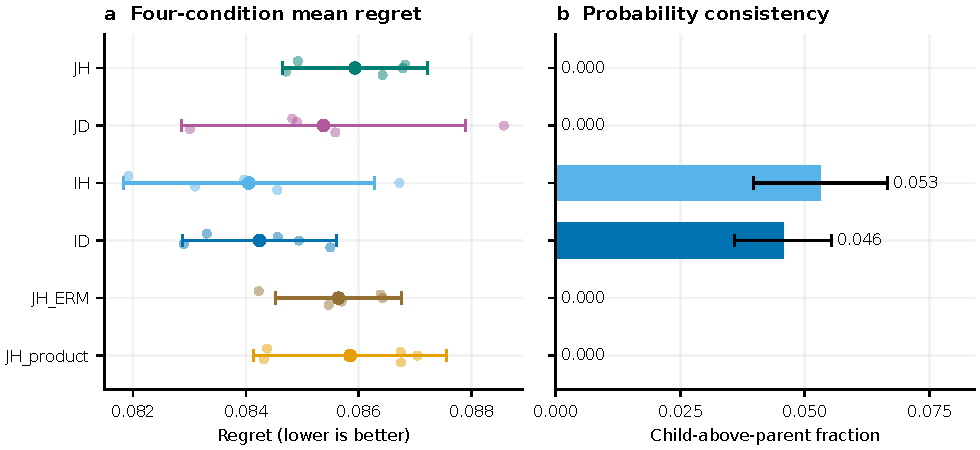
\includegraphics[width=\linewidth]{figures/figS1.pdf}
\caption{Structured synthetic regeneration. Panels show (a) four-condition mean regret and (b) child-above-parent violation rates for matched new variants. ID/IH use independent dense/hyperdimensional predictions; JD/JH use dependency factorization. JH\_ERM uses mean group risk; JH\_product scores marginal products from the JH checkpoint. Plot intervals are descriptive seed-t intervals. Text intervals cross seeds and 250 topology clusters using 2,000 paired bootstrap draws.}
\end{figure}

\newpage

\section*{S2. Direct candidate prediction and inexpensive alternatives}

A third study directly scored candidates without reconstructing fact probabilities. SCR mixes four candidate experts using observable global context. CAND\_CTX uses one expert with context; CAND\_LOCAL removes that context. Logistic regression (LOGIT) and a small denoising autoencoder (DAE) provide inexpensive fact-prediction comparisons. DAE pretraining reconstructs supplied, potentially corrupted observations; its targets are not oracle truth. Previously fitted ID and JH models were reevaluated unchanged on this study's new test pool.\par

Across the same four corruption mechanisms, SCR had mean regret 0.11152 versus 0.08644 for ID: paired difference +0.02508, 95\% crossed-bootstrap interval [0.02091, 0.02919]. SCR therefore underperformed ID, while improving descriptively over CAND\_CTX (0.12431), CAND\_LOCAL (0.12725), DAE (0.12873) and LOGIT (0.16455). The secondary SCR-minus-CAND\_CTX difference was -0.01279 [-0.01595, -0.00970], with unequal parameter counts and no multiplicity adjustment.\par

On shadow candidates formed by requirement unions, adding requirements should not increase feasibility probability; SCR violated this ordering in 41.153\% of comparisons, versus zero for the product-based DAE, LOGIT, ID and JH scores. Unions contained up to ten requirements, whereas training candidates had two to five. This is an informative query-length stress test, not proof that these violations caused the regret gap. Direct heads have no fact posterior; missing fact-coherence metrics do not mean zero semantic error.\par

All 25 newly fitted models reached the 40-epoch limit; selected checkpoints were at epochs 36–39, counted from zero. Convergence was not established. Thirty no-feasible snapshots remained in regret but not eligible recall. No synthetic weights transferred to the captured-flow experiments.\par

\begin{figure}[H]
\centering
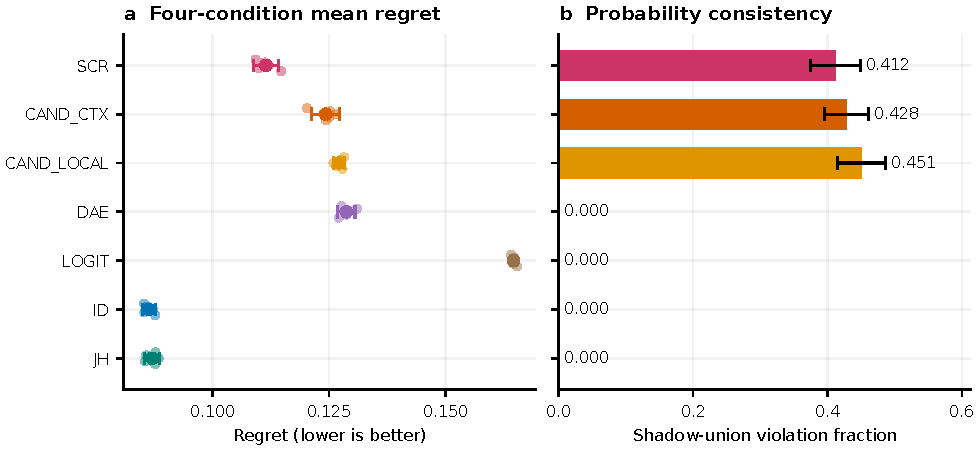
\includegraphics[width=\linewidth]{figures/figS2.pdf}
\caption{Direct candidate and inexpensive models. Panels show (a) four-condition mean regret and (b) added-requirement monotonicity violations on shadow-union candidates. Lower is better for both metrics. Error bars are descriptive intervals across five seeds; the primary SCR-versus-ID interval in the text crosses seeds and topology clusters. This study uses a separate fresh test pool from Figure S1.}
\end{figure}

\newpage

\section*{S3. Captured-flow protocol and optimization diagnostics}

CTU-13 [8] records controlled botnets in university traffic. Only From-Normal/From-Botnet rows enter: 799,777/19,976,700 (4.00\%). Training uses 442,084 flows (captures 1–8, 13); validation 214,880 (capture 9); testing 142,813 (captures 10–12). Training flows complete before validation, and validation before testing. Hosts can recur. Capture 12 contains NSIS.ay, absent from training; captures 10–11 contain Rbot. Reference numbering follows the main manuscript.\par

Graphs connect endpoint-sharing flows within 32-flow windows formed after label filtering. Fourteen features and fourteen availability masks omit numerical endpoint identities, times and capture identifiers. Training statistics standardize the first six features; inputs are clipped to [-5, 5]. Completed-flow classification is retrospective, not packet-causal or course-of-action evaluation.\par

Each training window is assigned once to clean, 20\% missing or 20\% centroid-replacement conditions in a cycle. Missingness clears features and masks; replacement substitutes the training-normal centroid for selected observed coordinates among the first eight, preserving categorical flags. Both preserve endpoints. Checkpoints minimize mean validation BCE plus Brier loss over these conditions. Clean-validation F1 chooses thresholds, favoring the highest tie, fixed across test conditions.\par

\begin{center}
\fontsize{9.5}{11}\selectfont
\renewcommand{\arraystretch}{1.12}
\setlength{\tabcolsep}{4pt}
\begin{tabularx}{\linewidth}{@{}>{\hsize=.84\hsize\raggedright\arraybackslash}X>{\hsize=1.16\hsize\raggedright\arraybackslash}X@{}}
\toprule
\textbf{Setting} & \textbf{Value} \\
\midrule
Device / framework & NVIDIA RTX 5000 Ada / PyTorch 2.9.1+cu128, CUDA 12.8 \\
Seeds / optimizer & 11, 23, 37, 51, 71 / AdamW \\
Learning rate / decay / supervised gradient clip & 0.001 / 0.0001 / 5 \\
Batch / supervision / stopping patience & 256 windows / at most 40 epochs / 8 epochs \\
New graph variants: parameters / pretraining & 121,643 / 5 epochs; EDGE\_DENSE uses none \\
\bottomrule
\end{tabularx}
\end{center}

New fits and thresholds were frozen before test inference; nine imported baselines remain unchanged. Consistency adds training passes despite matching parameter counts, and its original view can be corrupted.\par

\begin{figure}[H]
\centering
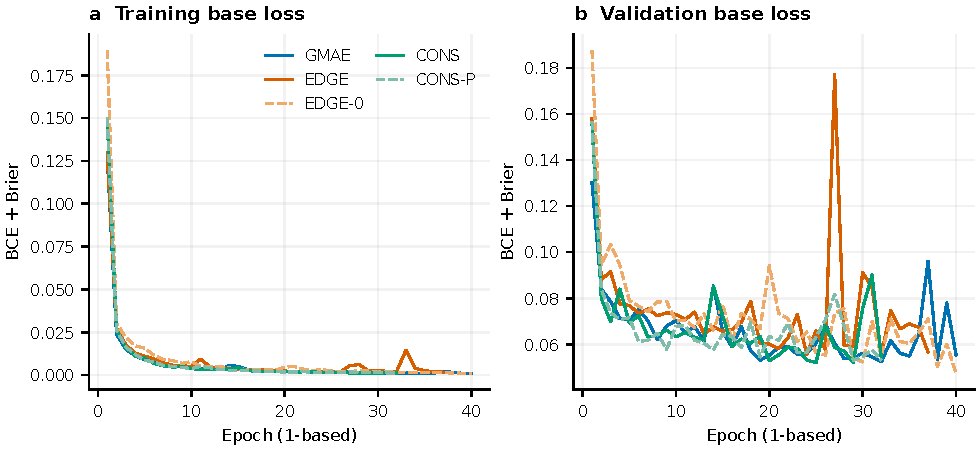
\includegraphics[width=\linewidth]{figures/figS3.pdf}
\caption{Optimization diagnostics. Curves show supervised BCE plus Brier loss, excluding consistency penalties. Baseline curves are unchanged. Each epoch averages seeds still represented after stopping; changing seed composition can affect the tail. These curves establish neither convergence nor equal training computation.}
\end{figure}

\newpage

\section*{S4. Paired uncertainty, controls and evidence checks}

Clean capture-macro AP differences versus GMAE were +0.01580 for EDGE\_GMAE and +0.00518 for CONS\_GMAE. Their ordinary 95\% intervals were [0.00097, 0.03710] and [-0.00184, 0.01441]. The respective 97.5\% marginal intervals, applying a nominal two-comparison Bonferroni adjustment, were [-0.00036, 0.04321] and [-0.00257, 0.01639]. Neither adjusted interval excludes zero; neither superiority nor equivalence is established. Prior inspection of these test captures makes the follow-up exploratory.\par

A shared paired bootstrap crossed model seeds with contiguous 64-window blocks within each fixed capture: 60, 6 and 5 blocks for captures 10, 11 and 12. It recomputed tie-aware AP with equal capture weights for 1,000 draws; no zero-positive draws were rejected. Individual flows were not treated as independent replicates, and captures were not resampled as a population of organizations. Small block populations and test reuse limit inference.\par

EDGE's mean gains were +0.00079, +0.04242 and +0.00420 by capture, concentrating the effect in capture 11. The no-pretraining EDGE\_DENSE control had the largest clean mean AP (0.99500), compared with EDGE\_GMAE (0.99411). At 50\% artificial missingness, their AP values were 0.95360 and 0.95962; these are descriptive secondary comparisons. CONS\_PRE (0.98272 clean AP) was close to CONS\_GMAE (0.98348). CONS\_PRE changes both view count and latent alignment relative to GMAE, so it does not isolate alignment's contribution.\par

Evidence checks covered 975 evaluation archives, 6,825 recomputed metrics and 65 checkpoint hashes. Seventy-five checkpoint replays reproduced 3,570,325 model-flow predictions exactly. Calibration counts include 46,414,225 repeated model-flow predictions, not that many independent flows. Only reliability-bin assignment and display clip 321 scores within 1.19e-7 above one; raw ranking metrics remain unchanged. Common-session host-wall median latency was 2.374/2.929/2.381 ms per window for GMAE/EDGE/CONS, including decoded-input transfer and graph construction but excluding capture ingestion and flow completion.\par

\begin{figure}[H]
\centering
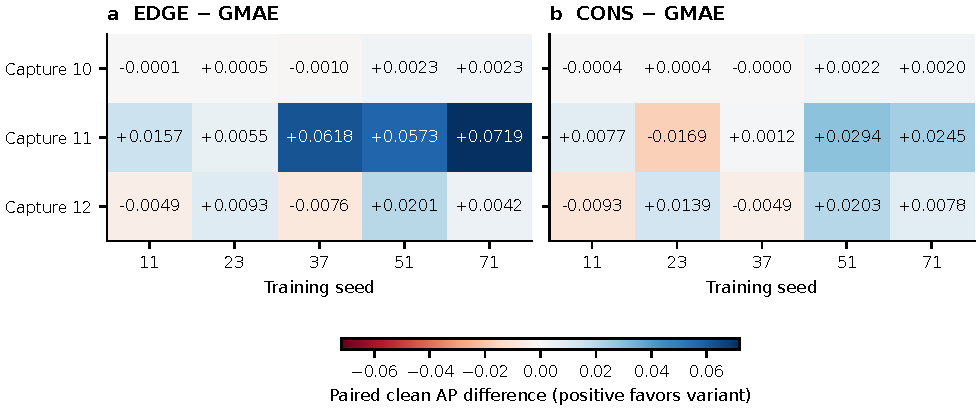
\includegraphics[width=\linewidth]{figures/figS4.pdf}
\caption{Paired seed effects on fixed captures. Capture-specific paired AP differences reveal seed variability and the concentration of EDGE's gain in capture 11. Seed averages are descriptive repeated fits on the same captures, not independent organizations. This figure complements the crossed seed/time-block intervals rather than providing an additional adjusted superiority test.}
\end{figure}

\end{document}
